\chapter{Design of OXC Scheduling\label{chap:design}}

\section{Open-Extension Container Structure\label{sec:design_oxc}}
Linux scheduling is runqueue, \texttt{struct rq}, centered and each 
scheduling class implements a set of interfaces to deal with the 
runqueue structure. In mainline Linux, \texttt{struct rq} is a per CPU 
structure. Each scheduling class defines its scheduling operations (
enqueue, dequeue, etc.) with this per CPU runqueue. On Multiple processor
platforms, tasks can migrate among different runqueues, also depending
on behaviours defined in a specific scheduler. In other words, on each CPU, 
a scheduling system is built up based on the associated runqueue.
Different per CPU scheduling systems cooperate with each other by task 
migrating operations defined by specific scheduling classes and construct 
the system level scheduling. One question raised here could be what if there
are extra runqueues and how they can be utilized. Ideally, suppose there is 
one extra runqueue, each scheduler can still use it as the scheduling 
parameter and a scheduling system can be built around it. If there are 
more than one extra runqueues, they can form a pseudo system level 
scheduling system.   

Extended from the above idea, a data structure named Open-Extension 
Container(OXC) is proposed in Linux kernel, shown in figure~\ref{fig:oxc}.
\begin{figure}[htbp]
        \centering
        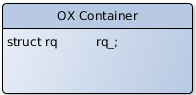
\includegraphics[width=0.5\textwidth]{images/oxc}
        \caption{Open-Extension Container}
        \label{fig:oxc}
\end{figure}
The ox container is designed as an abstract data structure; that is, any data
structure contains a \texttt{struct rq} runqueue inside can be called the ox
container. After bringing this new data structure into the kernel, there is 
not only per CPU runqueues in the system now, but also per oxc runqueues.

\section{The oxc scheduling\label{sec:design_oxc_scheduling}}
As there are extra per oxc runqueues besides 
per CPU ones in a system, they can be candidates passed as parameters to 
scheduling operations. From the standpoint of a scheduler, it manages a task 
over the runqueue according to implementation details in the scheduling class, 
and as long as a runqueue parameter is provided for its scheduling operations, 
the scheduler does not care whether it is associated with a CPU or from an ox 
container. So, as a oxc local runqueue is passed to hooks of scheduling 
classes, \textbf{tasks would enqueue, operate and dequeue on a per ox 
container runqueue}. This is called \textbf{the oxc scheduling}. The task 
enqueued in an ox container's local runqueue is called an oxc task. Of 
course, an oxc task can be a normal task or a RT task. For tasks or 
schedulers, the ox container behaves as a virtual CPU equipped with its
own runqueue.

\subsection{Scheduling routes in oxc enabled Linux 
\label{sec_design_oxc_routing}}

For tasks and scheduling classes, there is no difference between a per CPU 
and per container runqueue. This will be clearly shown when we see the 
scheduling route under the oxc scheduling. Previously, we saw
the path which relates each task with the per CPU runqueue it runs.
Figure~\vref{fig:cfs_routing_tg} is the scheduling route for a task under 
CFS scheduling when \texttt{CONFIG\_FAIR\_GROUP\_SCHED} is set; figure~ 
\vref{fig:rt_routing_tg} is the shceduling route under RT scheduling when 
RT group scheduling is enabled; figure~\vref{fig:routing_no_tg} is the 
scheduling route for a task without task group scheduling.
Now we are going to extend the scheduling routes in Linux for 
the oxc scheduling. As for how to connect different components and 
build such routes in Linux kernel, it is the content in 
chapter~\ref{chap:impl}.

When the oxc scheduling joins the system, original scheduling routes
will be extended. Nevertheless, it's very natural to adapt Linux 
scheduling routes to the oxc scheduling.
Figure~\ref{fig:oxc_fair_tg} shows the extended sheduling route for CFS
scheduling with \texttt{CONFIG\_FAIR\_GROUP\_SCHED} enabled. The only
change in this route is that for an oxc task, the terminal of the path 
will be a per ox container runqueue instead of its per CPU counterpart.
Figure~\ref{fig:oxc_rt_tg} shows the scheduling route for RT scheduling 
with \texttt{CONFIG\_RT\_GROUP\_SCHED} set; the situation is similar to 
CFS scheduling case we just saw. In fact, the same path is used to lead
a task to its per CPU or ox container runqueue. This means that the same 
codes can still be used to find both kinds of runqueues.

\begin{figure}[htbp]
\begin{center}
	\subfigure[The route for CFS scheduling] {
        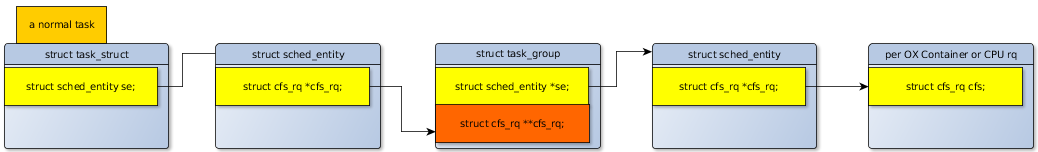
\includegraphics[height=2.5cm, width=\textwidth]{images/cfs_scheduling_scheme_tg_oxc}
        \label{fig:oxc_fair_tg}
	}
	\subfigure[The route for RT scheduling] {
        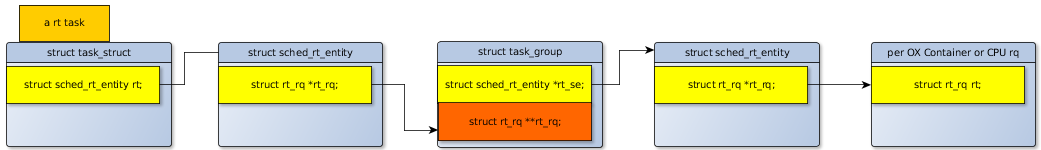
\includegraphics[height=2.5cm, width=\textwidth]{images/rt_scheduling_scheme_tg_oxc}
        \label{fig:oxc_rt_tg}
	}
\end{center}
	%\end{subfigure}
	\caption{Extended scheduling routes with task group scheduling}
	\label{fig:scheduling_route_oxc}
\end{figure}

In section~\ref{sec:LinuxSched_cfs}, we introduce that when task group
scheduling is not enabled, a macro \texttt{task\_rq} is used to associate
a task to its runqueue. The \texttt{task\_rq} is defined as follows:
\begin{lstlisting}
#define task_rq(p)              cpu_rq(task_cpu(p))
\end{lstlisting}
This macro can only return the dedicated rq for the CPU where the task is 
currently running on. So, when task group scheduling is not enabled, in 
order to merge oxc scheduling in the system, a new path leading a task 
to a runqueue is needed, shown in figure~\ref{fig:oxc_task_no_tg}. 
This route has two branches. When both RT and CFS group scheduling are not
enabled, these two paths coexist for a task since the 
\texttt{struct task\_struct} (listing~\ref{lst:task_struct}) embeds 
both RT and CFS entities. Also for this reason, when both
\texttt{CONFIG\_FAIR\_GROUP\_SCHED} and \texttt{CONFIG\_RT\_GROUP\_SCHED}
are set, the two routes in figure~\ref{fig:scheduling_route_oxc} originate
from a task at the same time too.
\begin{figure}[htbp]
        \centering
        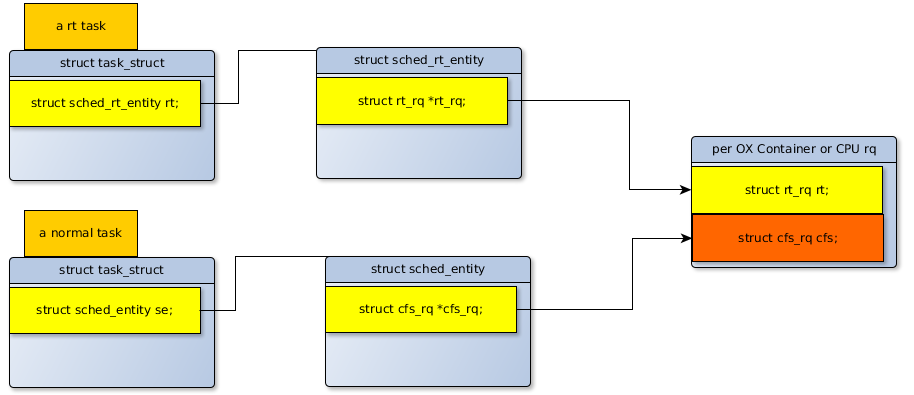
\includegraphics[width=\textwidth]{images/oxc_task_no_tg}
        \caption{Extended scheduling route without task group scheduling}
        \label{fig:oxc_task_no_tg}
\end{figure}

\subsection{Features of the oxc scheduling\label{sec_design_oxc_features}}

The first feature of oxc scheduling is that it is compatibe with Linux's
modular scheduling design. Tasks dealt by the RT scheduler or Completely Fair
Scheduler can naturally work under the oxc scheduling system. 
When there is new scheduling algorithm implemented in Linux kernel, 
like the case in \emph{sched\_deadline} patch we mentioned before, the
new scheduler has to fulfil details behind scheduling interfaces in 
\texttt{struct sched\_class}. Again, for each shceduling class, they do not
care whether a per CPU or per container runqueue is passed to its 
interfaces as the input, and the new scheduling class can also work under 
oxc scheduling. So, the ox container structure is {\bf open to extension}; 
this is where its name comes from.

When there is only per CPU runqueues, each scheduling operation defined 
in \texttt{struct sched\_class} will affect all tasks in the CPU. The
oxc scheduling provides another opportunity to restrict the influence of
a scheduling class in a fine grained scale. Now, the span to apply a 
scheduler can be controlled in the unit of an ox container. 

\section{Movtivation for oxc scheduling framework}
In section~\ref{sec:RelatedWork}, we see that, based on Linux, CPU bandwidth 
control can be applied in the level of single tasks or task groups which 
are scheduled by some policies. Such controls can be real-time or non real-time.
One obervation is that there does not exist a mechanism that can
control CPU bandwidth for all kinds of tasks as a whole without requirement of
a task' scheduling details. 

Suppose there is an ox container, different schedulers can use it to enqueue,
operate, and dequeue their tasks. If a fraction of CPU bandwidth can be allocated
to this ox container, all kinds of tasks inside the container will use it as if
running on a less powerful machine. This is the oxc solution to the CPU bandwidth 
control for general types of tasks.

Based on this idea, we develop an oxc scheduling framework in Linux that can 
realize hierarchical multi-processor reservation for tasks without requiring 
scheduling policies. 
%The oxc framework is not a scheduler. Although it cooperates with
%different scheduling classes, its pure responsibility is managing CPU power
%distribution. 
In the following chapter, details on how to implement 
this oxc scheduling framework in Linux kernel are described.

%%% Local Variables: 
%%% mode: latex
%%% TeX-master: "main"
%%% End: 
